% IJECES LaTeX Template
% IJECES Technical Support: Stephen Ward - sward@ferit.hr
% Requires XeLaTeX or LuaLaTeX typesetting engine
% Not complete. Please use the DOCX template (https://ijeces.ferit.hr/index.php/ijeces/libraryFiles/downloadPublic/236) as a guide to rest of the template (including reference formatting)

\documentclass[a4paper,10pt,twoside]{article}
\usepackage[a4paper, inner=20mm, outer=25mm, top=20mm, bottom=25mm]{geometry}
\usepackage{fancyhdr}
\pagestyle{fancy}
\fancyhf{}
\fancyfoot[LE,RO]{\thepage}
\renewcommand{\headrulewidth}{0pt}
\usepackage[english]{babel}
%\usepackage{fontspec}
\usepackage[T1]{fontenc}
\usepackage[utf8]{inputenc}
\usepackage{multicol}
\usepackage[explicit]{titlesec}
%\spanishdecimal{.}

\usepackage{lineno}
\usepackage{amsmath}
\usepackage{graphicx}
\usepackage{float}
\usepackage{booktabs}
\usepackage{multirow}
\usepackage{cite}
\usepackage{caption}
\usepackage{subcaption}
\captionsetup{font=small}
\usepackage[table]{xcolor}
\graphicspath{{imagenes/}{../Monografía/imagenes/}}
\usepackage{hyperref}


\setlength{\columnsep}{5mm}
%\setmainfont{Arial}
\titleformat{\section}
  {\normalfont\bfseries}{\thesection}{1em}{\MakeUppercase{#1}}
\titleformat{\subsection}
    {\normalfont\bfseries}{\thesubsection}{1em}{#1}
\titleformat{\subsubsection}
    {\normalfont\bfseries}{\thesubsubsection}{1em}{#1}

\begin{document}
\setlength{\parindent}{0ex}
{\fontsize{22}{0} \selectfont \textbf{Experimental Analysis of Body Shadowing Effects on a UWB Ranging System at 6.5 GHz}}
\begin{flushright}
{\fontsize{10}{0} \selectfont \textit{Original Scientific Paper}} %Please choose from the following Paper Categories: "Original Scientific Paper", "Review Paper", "Case Study" or "Preliminary Communication"
\end{flushright}

{\fontsize{12}{0} \selectfont \textbf{Danny Daniel Diaz Lopez}}

Author Affiliation: Universidad del Cauca

Address: Popayán-Cauca

E-mail: danieldiaz@unicauca.edu.co

\vspace{5mm}

{\fontsize{12}{0} \selectfont \textbf{Victor Quintero}}

Author Affiliation: Universidad del Cauca

Address: Popayán-Cauca

E-mail: vflorez@unicauca.edu.co

\vspace{5mm}

    \textbf{Abstract - }	\textit{Ultra-Wideband (UWB) is widely used in Indoor Positioning Systems (IPS) because its short pulses support accurate range estimation. In body-worn tracking, however, the human body can obstruct the radio link and introduce body-shadowing (BS) errors. This article reports an experimental characterization of BS in a 1D UWB ranging link operating at 6.5 GHz, a band for which fewer body-placement measurements have been reported than for 3-5 GHz systems. A fixed anchor and a body-worn tag were used to evaluate seven placements: head, chest, hip, wrist, hand, ankle, and knee. More than 100,000 independent Time-of-Flight (ToF) range samples were collected under Line-of-Sight (LOS) and Non-Line-of-Sight (NLOS) conditions in an indoor corridor and an outdoor open field. The results indicate a clear dependence on tag placement. Head placement yielded an MAE of 4.87 cm in outdoor LOS and 18.66 cm in indoor NLOS, while indoor LOS measurements varied across placements, with MAE values of 10.43 cm at the head, 16.49 cm at the chest, and 7.19 cm at the hip. Torso placements were the most affected under NLOS; the maximum reported MAE was 97.76 cm. Distribution fitting showed that NLOS absolute errors were better represented by a heavy-tailed log-normal model than by the Gaussian approximation often used in probabilistic ranging models. The indoor corridor also produced lower NLOS errors than the outdoor setting for several limb-mounted tags, suggesting that reflected components can partially preserve ToF observability when the direct path is blocked. These measurements provide experimental support for body-placement-aware and distribution-aware UWB ranging algorithms.}

\vspace{5mm}

\noindent\makebox[\linewidth]{\rule{\columnwidth}{0.4pt}}

\textbf{Keywords - }\textit{Ultra-Wideband (UWB), Body Shadowing, Time of Flight (ToF), Ranging Accuracy, 6.5 GHz, Ranging, Accuracy Performance.}

\noindent\makebox[\linewidth]{\rule{\columnwidth}{0.4pt}}

\setlength{\parindent}{3mm}
\begin{multicols}{2}
\section{Introduction}
\label{sec:introduction}
\input{introduccion.tex}

\section{Methodology}
\label{sec:methodology}
\input{metodologia.tex}

\section{Results}
\label{sec:results}
\input{resultados.tex}

\section{Analysis and Discussion}
\label{sec:discussion}
\input{discusion.tex}

\section{Conclusions}
\label{sec:conclusions}
\input{conclusiones.tex}

\section*{Acknowledgment}
The authors thank the School of Electronic and Telecommunication Engineering and the Master in Electronics and Telecommunications Engineering at the University of Cauca for the support provided during this research.

\section*{Conflict of Interest}
The authors declare no conflict of interest regarding the publication of this paper.

\section*{Data Availability Statement}
The data presented in this study and the validation datasets are available on GitHub at \url{https://github.com/danieldiaz-maestria/Sistema-de-\\
posicionamiento-2D}.

\bibliographystyle{ieeetr}
\bibliography{bibliografia/bibliografia.bib}

\vspace{1cm}
\section*{Biographies}

\noindent
\begin{minipage}[t]{0.3\linewidth}
    \centering
    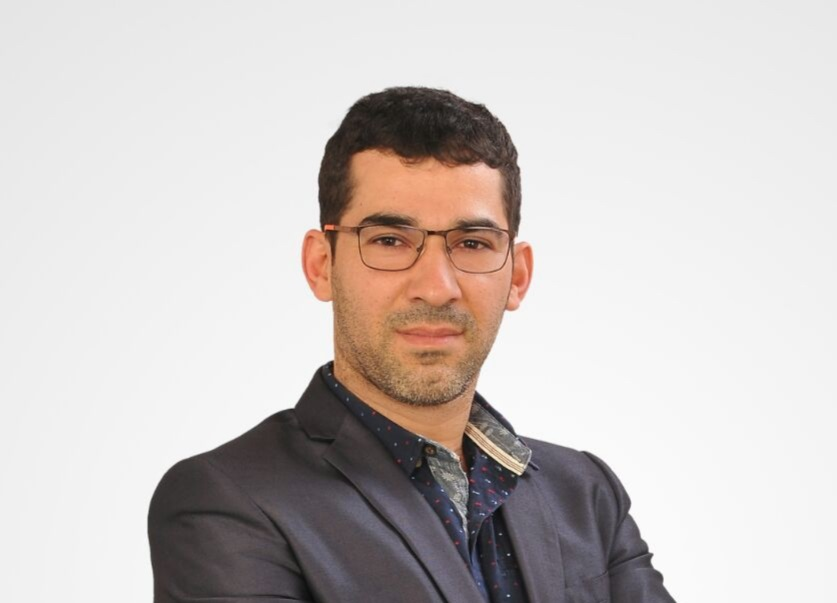
\includegraphics[width=0.8\linewidth]{imagenes/photo_danny.jpeg}
\end{minipage}%
\begin{minipage}[t]{0.7\linewidth}
    \textbf{Danny Daniel Diaz Lopez} received the B.S. degree in Electronics and Telecommunications Engineering from the University of Cauca, Popayán, Colombia. His research interests include wireless communications, indoor positioning systems, and signal processing.
\end{minipage}

\vspace{0.5cm}

\noindent
\begin{minipage}[t]{0.3\linewidth}
    \centering
    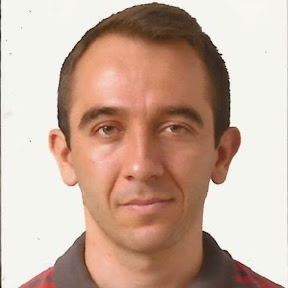
\includegraphics[width=0.8\linewidth]{photo_victor.jpeg}
\end{minipage}%
\begin{minipage}[t]{0.7\linewidth}
    \textbf{Victor Quintero} received the B.Sc. and M.Sc. degrees in electronics and telecommunications engineering from Universidad del Cauca, Popayán, Colombia, in 1999 and 2011, respectively, and the Ph.D. degree in electrical engineering from the Université de Lyon, Lyon, France, in 2018. He is currently an Assistant Professor at Universidad del Cauca. He is the Director of the GRIAL Research Group. His research interests span information theory, signal processing, and wireless communication systems. Dr. Quintero received the 2017 Best Ph.D. Thesis Award in the Domain of Information and Digital Societies from INSA de Lyon, Villeurbanne, France.
\end{minipage}
\end{multicols}
\end{document}
